% !TEX encoding = UTF-8
\documentclass[a4paper,12pt,titlepage=true, ngerman]{scrartcl}
%\usepackage{ngerman}, 
%\usepackage[ngerman]{babel}

\usepackage[utf8]{inputenc}
\usepackage[ngerman]{babel}
\usepackage[babel]{csquotes}

\usepackage[backend=biber, style=authoryear-comp, maxbibnames=3,
 isbn=false, doi=false, eprint=false, dashed=false]{biblatex}
 
\ExecuteBibliographyOptions{maxcitenames=2}

\bibliography{literature.bib}
\usepackage{hyperref}
%\hypersetup{
%colorlinks=true, linktocpage=false, pdfborder={0 0 0}, pdfstartview=FitV, 
%urlcolor=Black, linkcolor=Black, citecolor=Black, %pdfstartpage=3, 
%}
\usepackage{graphicx}

\usepackage{scrhack}
\KOMAoptions{BCOR=8mm}
%\KOMAoptions{toc=flat}
% \KOMAoptions{toc=graduated, toc=bibliography}

% \renewcommand*\sectfont{\rmfamily\mdseries\scshape}
\setkomafont{section}{\rmfamily\bfseries\LARGE}
% \setkomafont{sectionentry}{\rmfamily\bfseries\scshape\Large}
\setkomafont{subsection}{\rmfamily\bfseries\Large}
\setkomafont{subsubsection}{\rmfamily\bfseries\large}
%\setkomafont{chapter}{\rmfamily\bfseries\scshape\huge}
%  \setkomafont{partentry}{\rmfamily\bfseries\scshape}
% \setkomafont{chapterentry}{\rmfamily\bfseries\scshape}
\setkomafont{partentry}{\rmfamily\bfseries\scshape}
\setkomafont{part}{\rmfamily\bfseries\scshape\huge}
\setkomafont{partnumber}{\rmfamily\bfseries\scshape\huge}
\setkomafont{partentrypagenumber}{\rmfamily\bfseries\scshape}

\setkomafont{descriptionlabel}{\bfseries}

%  scrhack to fuck float error message

%%%%  for page head and foot %%%%%%%
\usepackage[automark]{scrpage2}
\pagestyle{scrheadings}
\KOMAoptions{headsepline=true}
\setheadsepline{.4pt}
\setkomafont{pageheadfoot}{\normalfont\normalcolor\upshape} 

\setcounter{tocdepth}{3}
\setcounter{secnumdepth}{4}

\usepackage[T1]{fontenc} % to make Sa\"ibi searchable
\usepackage[protrusion=true,expansion=true]{microtype}
% \usepackage{microtype}
% \usepackage{setspace}\setstretch{1.2}



% \usepackage{lmodern} 


%  \usepackage{palatino}\linespread{1.05}
 \usepackage{mathpazo}\linespread{1.05}  
\usepackage[scaled=.95]{helvet}
   \usepackage{courier}
   \usepackage[scaled]{berasans}
 
% \usepackage[bitstream-charter]{mathdesign}  %%%%%%%%%%%%%%%%%%%%%  FINAL VERSION %%%%%%%%%%%%%%%%%%%%%%%%%%%%%%%

%\usepackage[style=authoryear,
% 	maxnames=1,
%  	maxbibnames=99,                  %%%%%%%%     TODO  activate
% uniquename=init
%]{biblatex}

\usepackage{calc}
\usepackage{ifthen}

\usepackage{tikz}
\usetikzlibrary{shapes,arrows}

\tikzstyle{task} = [diamond, draw, fill=green!20, 
    text width=4.5em, text badly centered, node distance=2cm, inner sep=0pt]
\tikzstyle{comp} = [rectangle, draw, fill=blue!20, 
    text width=5em, text centered, rounded corners, minimum height=4em, node distance=2cm]
\tikzstyle{line} = [draw, -latex']
\tikzstyle{line2} = [draw, double, -latex']
\tikzstyle{human} = [draw, ellipse,fill=red!20, text width=5em, text centered, node distance=2cm,
    minimum height=3em]
\tikzstyle{decision} = [diamond, draw, fill=green!20, 
    text width=4.5em, text badly centered, node distance=3cm, inner sep=0pt]
\tikzstyle{block} = [rectangle, draw, fill=blue!20, 
    text width=5em, text centered, rounded corners, minimum height=4em]
\tikzstyle{cloud} = [draw, ellipse,fill=red!20, text width=5em, text centered, node distance=3cm,
    minimum height=2em]

% % Pie chart
\newcommand{\slice}[4]{
  \pgfmathparse{0.5*#1+0.5*#2}
  \let\midangle\pgfmathresult

  % slice
  \draw[thick,fill=black!10] (0,0) -- (#1:1) arc (#1:#2:1) -- cycle;

  % outer label
  \node[label=\midangle:#4] at (\midangle:1) {};

  % inner label
  \pgfmathparse{min((#2-#1-10)/110*(-0.3),0)}
  \let\temp\pgfmathresult
  \pgfmathparse{max(\temp,-0.5) + 0.8}
  \let\innerpos\pgfmathresult
  \node at (\midangle:\innerpos) {#3};
}

\usepackage{bchart}


\usepackage{setspace}
\onehalfspacing

% \usepackage{framed}

\usepackage{graphicx}

\usepackage{ownstyle}

\usepackage{cleveref}


%###########################################################################
%%%%%%%%%%%%%%%%%%%%%%%%%%%%%%%%%%%%%%%%%%%%%%%%%%%%%%%%
%###########################################################################

\pagenumbering{roman}

\title{Dokumentation zur Arbeit von Gruppe 2 im Projekt ''Praxis der Digital Humanities''} % title
\author{Clemens Ahrens}

\begin{document}
\begin{titlepage}

\begin{center}

\vspace*{100pt}

\textbf{\Large{Dokumentation zur Arbeit von Gruppe 2 im Projekt ''Praxis der Digital Humanities''}}% title

\vfill

Schriftliche Dokumentation

im Seminar

\emph{Praxis der Digital Humanities}


Leitung:

\textbf{Prof.\ Dr.\ Caroline Sporleder}% leitung

WiSe 2014/2015% semester

\bigskip
\bigskip

an der Universität Trier

Fachbereich II

\bigskip

\bigskip

Verfasser:


\textbf{Clemens Ahrens}

Matrikelnummer: 1116125

\textbf{Andre} %TODO

Matrikelnummer: xxxxxx

\textbf{Christopher Michels} %TODO

Matrikelnummer: 1007830


% \bigskip

\vfill

\end{center}

\end{titlepage}


%###########################################################################
%%%%%%%%%%%%%%%%%%%%%%%%%%%%%%%%%%%%%%%%%%%%%%%%%%%%%%%%
%###########################################################################

\thispagestyle{empty}
\subsection*{Erklärung}
Hiermit erkläre ich, dass ich die Hausarbeit selbstständig
verfasst und keine anderen als die angegebenen Quellen und Hilfsmittel benutzt
und die aus fremden Quellen direkt oder indirekt übernommenen Gedanken als
solche kenntlich gemacht habe.

Die Arbeit habe ich bisher keinem anderen Prüfungsamt in gleicher oder
vergleichbarer Form vorgelegt. Sie wurde bisher nicht veröffentlicht.


\vspace{3cm}
\begin{center}
(Datum) \hspace{8cm} (Unterschrift)
\end{center}
% \left Datum
% \right Unterschrift


%###########################################################################
%%%%%%%%%%%%%%%%%%%%%%%%%%%%%%%%%%%%%%%%%%%%%%%%%%%%%%%%
%###########################################################################

\newpage

\microtypesetup{protrusion=false}
 \tableofcontents%[liststotoc]
\microtypesetup{protrusion=true}

% \newpage
% \listoffigures
% \listoftables


%###########################################################################
%%%%%%%%%%%%%%%%%%%%%%%%%%%%%%%%%%%%%%%%%%%%%%%%%%%%%%%%
%###########################################################################

\newpage

\listoffigures


%###########################################################################
%%%%%%%%%%%%%%%%%%%%%%%%%%%%%%%%%%%%%%%%%%%%%%%%%%%%%%%%
%###########################################################################

\newpage

\listoftables

%###########################################################################
%%%%%%%%%%%%%%%%%%%%%%%%%%%%%%%%%%%%%%%%%%%%%%%%%%%%%%%%
%###########################################################################

\newpage
\pagenumbering{arabic}

\section{Einleitung}\label{Einleitung} %TODO
 
Im Rahmen des Seminars \emph{Praxis der Digital Humanities} haben sich die einzelnen Gruppen vorgenommen, 
ein Werkzeug zu entwickeln, das literaturwissenschaftliche Arbeit unterstützt. 
Diese Hilfssoftware soll dazu dienen, die stereotype Darstellung von einzelnen Personen oder Gruppen in Texten zu analysieren 
und zu visualiseren. 
Vor diesem Hintergrund baut die hier vorgestellte Arbeit der zweiten Gruppe auf den Vorverarbeitungsschritten der ersten Gruppe auf 
und fügt für die drei Werke \emph{Uncle Tom's Cabin}  \autocite[]{chris_uncle}, 
\emph{To Kill a Mockingbird}  \autocite[]{chris_bird} und 
\emph{The Adventures of Huckleberry Finn: Tom Sawyer} \autocite[]{chris_adventures} \textbf{Informationen zu Koreferenzketten} hinzu. 
Auf diese Weise trägt die Gruppe zwei neben der \emph{Named Entity Recognition} als Vorverarbeitungsschritt der ersten Gruppe dazu bei, 
dass die Protagonisten erkennbar werden und so von der dritten Gruppe auf ihre literarische Darstellung hin untersucht werden können.

Im Folgenden werden \emph{Bart 2.0}, \emph{DCoref} und \emph{Reconcile} als Softwarew vorgestellt, 
die zunächst für die Koreferenzresolution in Betracht gezogen wurden. 
Dieser Ausgangspunkt stellte die zweite Gruppe vor die Aufgabe, die einzelnen Werkzeuge zu bewerten und zu vergleichen. 
Nach der Zusammenfassung des Verlaufs und der Ergebnisse dieses Vergleichs wird anschließend knapp dargestellt, 
welche Formatierungsanforderungen für die Schnittstellen zu den anderen Gruppen beachtet werden mussten 
und wie kapitelbezogene Koreferenzketten zu kapitelübergreifenden Ketten zusammengefasst wurden. 
Zuletzt folgt ein Beispiel für die Verwendung und die Ausgabe eines der Werkzeuge.


%###########################################################################
%%%%%%%%%%%%%%%%%%%%%%%%%%%%%%%%%%%%%%%%%%%%%%%%%%%%%%%%
%###########################################################################

\newpage

\section{Ansätze zur Koreferenzresolution}\label{Ansätze zur Koreferenzresolution} %TODO


%###########################################################################

\subsection{BART 2.0}

% !TEX encoding = UTF-8
\subsubsection{Steckbrief}
Analysiert wurde \href{http://www.bart-anaphora.org/}{BART} in der Version 2.0, 
wie sie \href{http://www.bart-anaphora.org/release/bart-2.0.tar.gz}{hier} zu finden 
ist.
Es stehen dem Nutzer zwei Modi zur Nutzung zur Verfügung.
\begin{itemize}
\item BART-WebServer als end-to-end Blackbox Lösung
\item BART-full zum Trainieren eines neuen Modells
\end{itemize}
Erstere erzeugt aus einem Rohtext-Input einen Output, 
wie er in Abb.\ref{bart_webUI_output} zu sehen ist.
Hierfür werden verschiedene Verarbeitungsschritte durchgeführt. 
Diese analysieren jeweils unterschiedliche Ebenen in Syntax und Semantik. 
Beispielhaft hierfür soll der Output der WebServer-Anwendung für die Wortebene in 
Listing\ref{output:bart_word} stehen.

\begin{lstlisting}[label=output:bart_word, name=words.xml, language=xml, caption=BART-Output der Wortebene]
?xml version="1.0" encoding="UTF-8"?>
<!DOCTYPE words SYSTEM "words.dtd">
<words>
  <word id="word_1">Late</word>
  <word id="word_2">in</word>
  <word id="word_3">the</word>
  <word id="word_4">afternoon</word>
  ...
</words>
\end{lstlisting}
Der Output auf Koreferenzebene im XML-Format ist exemplarisch in 
Listing\ref{output:bart_response} dargestellt.
Hierbei ist die Koreferenzkette ,,a low man'' aus Abb.\ref{bart_webUI_output} in dem 
Attribut \lstinline[language=XML]{coref_set="set_4"} kodiert.

\begin{lstlisting}[label=output:bart_response, name=XXX_response_level.xml, language=xml, caption=BART-Output der Koreferenzebene]
<markables>
  ...
  <markable id="markable_51" span="word_120..word_122" coref_set="set_4" min_ids="word_120..word_122" mmax_level="response"/>
  <markable id="markable_13" span="word_128" coref_set="set_4" dir_antecedent="markable_51" mmax_level="response"/>
  <markable id="markable_0" span="word_128..word_129" coref_set="set_0" min_ids="word_128..word_129" mmax_level="response"/>
  ...
</markables>
\end{lstlisting}

\begin{figure}[ht]
\begin{center}
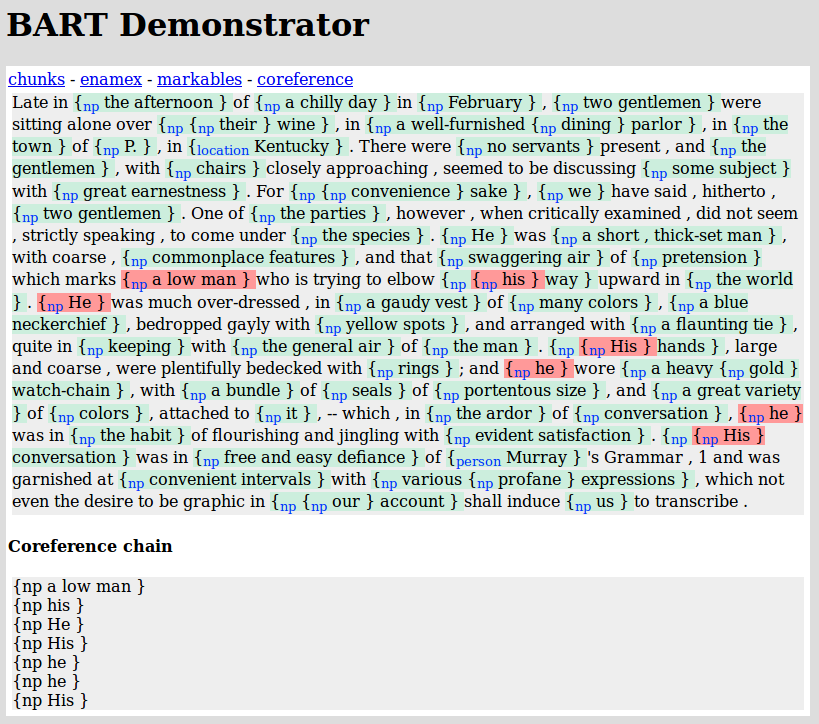
\includegraphics[width=12cm]{./img/cle/bart_webUI_output.png}
 % bart_webUI_output.png: 819x724 pixel, 72dpi, 28.89x25.54 cm, bb=0 0 819 724
\caption{BART 2.0: Output für WebInterface der Blackbox Version}
\label{bart_webUI_output}
\end{center}
\end{figure}

\subsubsection{Probleme}

\noindent
Neben der Blackbox-Version bietet BART noch eine Terminalapplikation, 
die zum Trainieren neuer Modelle genutzt werden kann.
Hierfür stehen verschiedene interne Konfigurationsdateien zur Verfügung,
die sich jedoch auf die Weiterverarbeitung beziehen und nicht den erwarteten
Input modifizieren.

Da im Projekt die Verarbeitung von Output des Stanford Parsers gewünscht war,
und wir daher auch innerhalb unserer Gruppe von der Verwendung des MMAX-Formats 
Abstand genommen haben, wurde von der Konvertierung in dieses Format abgesehen.
Eine erste Analyse der Koreferenzketten, die die WebServer-Version von BART ausgab,
unterstützte diese Entscheidung ebenfalls.




%###########################################################################

\subsection{DCoref}

% !TEX encoding = UTF-8

\subsubsection{Steckbrief}

Das Werkzeug \emph{DCoref} ist ein deterministisches Modul zur Koreferenzresolution und ist Teil der \emph{Stanford CoreNLP}. Für die Verwendung dieses Moduls ist vorausgesetzt, dass andere Module vorher auf die Eingabedaten angewendet worden sind \autocite[]{chris_stanford_dcoref}. Die Module für Wortart- und Lemmabestimmung sowie Named Entitiy Recognition und für einen Parser müssen als sogenannte Annotatoren beim Verwenden der \emph{Stanford CoreNLP} wie in Listing \ref{dcoref:required_annotators} angebeben werden.

\begin{lstlisting}[label=dcoref:required_annotators, language=Java, caption=Angabe vorausgesetzter Annotatoren in Java]
//	configure properties for pipeline of the Stanford CoreNLP
Properties properties = new Properties();
properties.setProperty("annotators", 
		"pos, lemma, ner, parse, dcoref");
//	[...] set more properties and instantiate pipeline
StanfordCoreNLP pipeline = new StanfordCoreNLP(properties);
\end{lstlisting}

\noindent Außerdem ist \emph{DCoref} grundsätzlich ein zweistufiges Modul, das mit mehreren sogenannten Sieben arbeitet. Die erste Stufe legt großen Wert auf Recall und dient der Identifizierung von vorhandenen \emph{mentions} (\hyphenquote{UKenglish}{A mention is an observed textual reference to a latent real-world entity. Mentions are associated with nodes in a parse tree and are typically realized as NPs.} \autocite[S. 385 f.]{chris_haghighi}). Die zweite Stufe siebt das Ergebnis der ersten Stufe mit mehreren Sieben aus, wobei die Siebe absteigend gemäß ihrer Precision-Werte nacheinander angewendet werden \autocite[S. 28 f.]{chris_leeetal}. 

Es gibt noch eine weitere optionale Stufe, die das Endergebnis der zweiten Stufe noch weiterverarbeitet. Dabei werden Koreferenzketten mit nur einem Element entfernt und auch \emph{mentions} entfernt, die als appositive oder copulative Textelemente auftauchen \autocite[29]{chris_leeetal}. Dieses Stufe ist optional, weil fälschlicherweise aufgeführte \emph{mentions} die Score-Werte für \emph{DCoref} nicht so sehr negativ beeinflussen wie gänzlich fehlende relevante \emph{mentions} \autocite[32]{chris_leeetal}.


\subsubsection{Probleme}

Bei der Verwendung von \emph{DCoref} sind vor allem fehlende Informationen aufgefallen. Obwohl die Dokumentation auf der Homepage des Moduls \autocite[]{chris_stanford_dcoref} zunächst sehr ausführlich erscheint, verweist sie auf Download-Links, die auf Archive verweisen, in denen Dateien fehlen, wie z.B. ein Perl-Skript, das für den CoNLL-Scorer benötigt wird ist nicht vorhanden. Dieses Skript konnte man jedoch nach einer kurzen Suche leicht finden. Obwohl angegeben ist, dass man den Pfad zu diesem Skript als Option angeben kann, scheint diese Option ignoriert zu werden und ein im Code fest vorgegebener Pfad wird trotzdem verwendet. Außerdem wird nicht angegeben, dass man neben einer Standardinstallation von Perl ein bestimmtes Paket (\emph{Algorithm-Munkres}) nachinstallieren muss, da sonst das Skript nicht ausführbar ist. Versucht man, dieses Skript trotzdem über die \emph{Stanford CoreNLP} auszuführen, erfährt man nichts von dieser speziellen Fehlerursache.

Neben der Reproduktion der Score-Werte, die für die \emph{CoNLL Shared Task 2011} bestimmt wurden, sind noch andere Optionen für den in das Modul \emph{DCoref} integrierten Scorer aufgelistet, z.B. die Verwendung des Scorers für Daten im MUC6- oder ACE2004-Format. Jedoch musste der Versuch, diesen Scorer für das MUC6-Format beim Vergleichen der Ansätze zur Koreferenzresolution zu verwenden, aus Zeitgründen ergebnislos aufgegeben werden, da die Verwendung auch nach mehreren Versuchen nicht so funktioniert hat, wie die Dokumentation es angedeutet hat. 


%###########################################################################

\subsection{Reconcile} %TODO


%~~~

\subsubsection{Steckbrief} %TODO


%~~~

\subsubsection{Probleme} %TODO


%###########################################################################
%%%%%%%%%%%%%%%%%%%%%%%%%%%%%%%%%%%%%%%%%%%%%%%%%%%%%%%%
%###########################################################################

\newpage

\section{Verlauf der Gruppenarbeit}\label{Verlauf der Gruppenarbeit} %TODO


%###########################################################################

\subsection{Vergleich}%TODO


%~~~

\subsubsection{Ausgangssituation}

Wie bereits erwähnt, wurde \emph{BART 2.0} für den Vergleich der Ansätze zur Koreferenzresolution als Kandidat verworfen. Übrig geblieben sind also \emph{DCoref} und \emph{Reconcile}. Das Ziel des Vergleichs war es, mit einem MUC-Scorer anhand der Werte Precision, Recall und F-Score den besseren der verbleibenden zwei Kandidaten zu finden. Um einen Goldstandard für den Vergleich der beiden Ansätze zu erhalten, wurde die erste Hälfte des ersten Kapitels aus \emph{Uncle Tom's Cabin} \autocite[]{chris_uncle} als Testdatensatz für eine manuelle Annotierung mit Unterstützung des dafür vorgesehenen Softwarewerkzeugs \href{http://mmax2.sourceforge.net/}{MMAX} verwendet. 


%~~~

\subsubsection{Probleme mit MMAX}%TODO

Probleme mit MMAX


%~~~

\subsubsection{Alternative Lösung}%TODO

Alternative Lösung \emph{DCoref} \autocite[S. 385 f.]{chris_haghighi}


%###########################################################################

\subsection{Formatierung}%TODO


%~~~

\subsubsection{DCoref}%TODO


%~~~

\subsubsection{Reconcile}%TODO

%###########################################################################

\subsection{Indizierung}%TODO



%% !TEX encoding = UTF-8
\subsubsection{Steckbrief}
Analysiert wurde \href{http://www.bart-anaphora.org/}{BART} in der Version 2.0, 
wie sie \href{http://www.bart-anaphora.org/release/bart-2.0.tar.gz}{hier} zu finden 
ist.
Es stehen dem Nutzer zwei Modi zur Nutzung zur Verfügung.
\begin{itemize}
\item BART-WebServer als end-to-end Blackbox Lösung
\item BART-full zum Trainieren eines neuen Modells
\end{itemize}
Erstere erzeugt aus einem Rohtext-Input einen Output, 
wie er in Abb.\ref{bart_webUI_output} zu sehen ist.
Hierfür werden verschiedene Verarbeitungsschritte durchgeführt. 
Diese analysieren jeweils unterschiedliche Ebenen in Syntax und Semantik. 
Beispielhaft hierfür soll der Output der WebServer-Anwendung für die Wortebene in 
Listing\ref{output:bart_word} stehen.

\begin{lstlisting}[label=output:bart_word, name=words.xml, language=xml, caption=BART-Output der Wortebene]
?xml version="1.0" encoding="UTF-8"?>
<!DOCTYPE words SYSTEM "words.dtd">
<words>
  <word id="word_1">Late</word>
  <word id="word_2">in</word>
  <word id="word_3">the</word>
  <word id="word_4">afternoon</word>
  ...
</words>
\end{lstlisting}
Der Output auf Koreferenzebene im XML-Format ist exemplarisch in 
Listing\ref{output:bart_response} dargestellt.
Hierbei ist die Koreferenzkette ,,a low man'' aus Abb.\ref{bart_webUI_output} in dem 
Attribut \lstinline[language=XML]{coref_set="set_4"} kodiert.

\begin{lstlisting}[label=output:bart_response, name=XXX_response_level.xml, language=xml, caption=BART-Output der Koreferenzebene]
<markables>
  ...
  <markable id="markable_51" span="word_120..word_122" coref_set="set_4" min_ids="word_120..word_122" mmax_level="response"/>
  <markable id="markable_13" span="word_128" coref_set="set_4" dir_antecedent="markable_51" mmax_level="response"/>
  <markable id="markable_0" span="word_128..word_129" coref_set="set_0" min_ids="word_128..word_129" mmax_level="response"/>
  ...
</markables>
\end{lstlisting}

\begin{figure}[ht]
\begin{center}
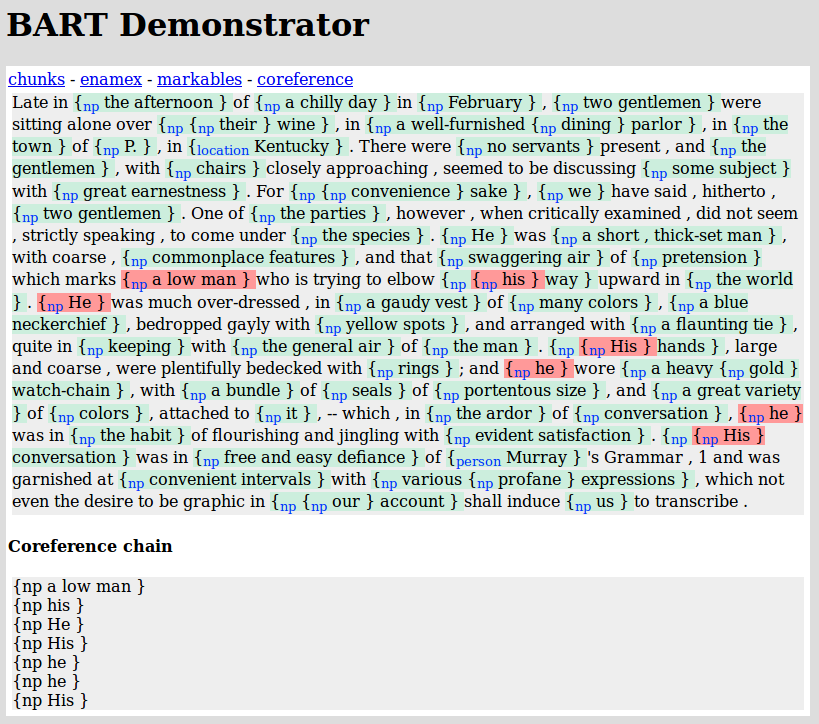
\includegraphics[width=12cm]{./img/cle/bart_webUI_output.png}
 % bart_webUI_output.png: 819x724 pixel, 72dpi, 28.89x25.54 cm, bb=0 0 819 724
\caption{BART 2.0: Output für WebInterface der Blackbox Version}
\label{bart_webUI_output}
\end{center}
\end{figure}

\subsubsection{Probleme}

\noindent
Neben der Blackbox-Version bietet BART noch eine Terminalapplikation, 
die zum Trainieren neuer Modelle genutzt werden kann.
Hierfür stehen verschiedene interne Konfigurationsdateien zur Verfügung,
die sich jedoch auf die Weiterverarbeitung beziehen und nicht den erwarteten
Input modifizieren.

Da im Projekt die Verarbeitung von Output des Stanford Parsers gewünscht war,
und wir daher auch innerhalb unserer Gruppe von der Verwendung des MMAX-Formats 
Abstand genommen haben, wurde von der Konvertierung in dieses Format abgesehen.
Eine erste Analyse der Koreferenzketten, die die WebServer-Version von BART ausgab,
unterstützte diese Entscheidung ebenfalls.



%% !TEX encoding = UTF-8
\section{clemens\_code}\label{clemens_code}
%TODO headings for lstlistings
\lstset{language=Java} 
\begin{lstlisting}[caption=Main-Klasse der BuildIndex,label=code:Coref, name=Coref.java] 
import java.util.ArrayList;
import java.util.Map;

public class Coref {
	ArrayList<String> inFiles;
	String outFile;

	// parser for inputs
	void parseArgs(String[] args) {
		Integer iIdx = null;
		Integer oIdx = null;
		inFiles = new ArrayList<String>();

		// input must come before output ---
		for (int i = 0; i < args.length; i++) {
			if (args[i].equals("-i")) {
				iIdx = new Integer(i);
			} else if (args[i].equals("-o")) {
				oIdx = new Integer(i);
			}
		}
		if (iIdx != null & oIdx != null) {
			outFile = args[oIdx + 1];
			for (int i = iIdx + 1; i < oIdx; i++) {
				inFiles.add(args[i]);
			}
		} else {
			System.out.println("Usage: " + "\n"
					+ "java Coref -i <XmlFile> -o <NewFile>" + "\n"
					+ "Example (Linux): " + "\n"
					+ "java Coref -i ../Input/*.xml -o ../output.xml");
			System.exit(-1);
		}
	}

	public static void main(String[] args) {
		Coref coref = new Coref();
		coref.parseArgs(args);

		OutputWriter outputWriter = new OutputWriter(coref.getOutFile());

		// for each input XML: Analyze, build Maps of coreferences, pass to output XML
		try {
			for (String inFile : coref.getInFiles()) {
				InputAnalyzer inputAnalyzer = new InputAnalyzer(inFile);

				Map<String, Coreference> coreferences = inputAnalyzer
						.extractCoreferences();

				outputWriter.addCoreferences(coreferences);
			}
		} catch (Exception e) {

			e.printStackTrace();
		}

		// create output XML
		outputWriter.writeToFile();

	}

	public ArrayList<String> getInFiles() {
		return inFiles;
	}

	public String getOutFile() {
		return outFile;
	}
}
\end{lstlisting} 

\begin{lstlisting}[caption=Coreference-Klasse,label=code:Coreference, name=Coreference.java]
public class Coreference {
	String text;
	String chapId;
	Integer corefId;

	public Coreference(String text, String chapId, Integer corefId) {
		this.text = text;
		this.chapId = chapId;
		this.corefId = corefId;
	}

	public String getText() {
		return text;
	}

	public void setText(String text) {
		this.text = text;
	}

	public String getChapId() {
		return chapId;
	}

	public void setChapId(String chapId) {
		this.chapId = chapId;
	}

	public Integer getCorefId() {
		return corefId;
	}

	public void setCorefId(Integer corefId) {
		this.corefId = corefId;
	}

}
\end{lstlisting}

\begin{lstlisting}[caption=InputAnalyzer-Klasse,label=code:InputAnalyzer, name=InputAnalyzer.java]
import java.io.File;
import java.io.IOException;
import java.util.ArrayList;
import java.util.HashMap;
import java.util.List;
import java.util.Map;

import org.jdom.Document;
import org.jdom.Element;
import org.jdom.JDOMException;
import org.jdom.input.SAXBuilder;

public class InputAnalyzer {

	File infile;
	
	public InputAnalyzer(String filename) throws Exception {
		infile = new File(filename);
		if (!infile.exists()) {
			throw new Exception("File " + filename + " not found");
		}
	}

	public Map<String, Coreference> extractCoreferences() {
		Map<String, Coreference> map = new HashMap<String, Coreference>();

		// aufrufen des builders pro input
		SAXBuilder builder = new SAXBuilder();
		try {
			Document doc = builder.build(infile);

			// ---- Create list of <coreferences> & extract chapID
			Element root = doc.getRootElement();

			// extract argument chapter ID for output document
			String chapID = root.getAttribute("id").getValue();

			// jump to necessary level of sub elements
			Element corefs = root.getChild("coreferences");

			@SuppressWarnings("unchecked")
			List<Element> listcoref = corefs.getChildren("coreference");
			for (Element coref : listcoref) {
				String corefID = coref.getAttribute("id").getValue();

				// create list of mentions for each coreference chain
				@SuppressWarnings("unchecked")
				List<Element> listmention = coref.getChildren("mention");
				for (Element mention : listmention) {
					if (null == mention)
						continue;
					
					// search for "representative" mention
					String s = mention.getAttributeValue("representative");
					if (null == s || !s.equals("true"))
						continue;

					// extract XML element <text> for output document
					String text = mention.getChildText("text");

					// build new Coreference element with needed attributes &
					// turn corefID to Integer
					Coreference coreference = new Coreference(text, chapID,
							Integer.parseInt(corefID));
					map.put(text, coreference);

				}
			}
		} catch (JDOMException | IOException e) {
			// TODO Auto-generated catch block
			e.printStackTrace();
		} catch (NumberFormatException e) {
			System.err.println("Error while parsing corefID: \n"
					+ e.getMessage());
		}

		return map;

	}

}
\end{lstlisting}
\begin{lstlisting}[caption=OutputWriter-Klasse der BuildIndex,label=code:OutputWriter, name=OutputWriter.java]
import java.io.File;
import java.io.FileOutputStream;
import java.io.IOException;
import java.util.ArrayList;
import java.util.HashMap;
import java.util.Map;
import java.util.Set;

import org.jdom.Document;
import org.jdom.Element;
import org.jdom.output.Format;
import org.jdom.output.XMLOutputter;

public class OutputWriter {

	File outFile;
	Map<String, ArrayList<Coreference>> multiMap;

	public OutputWriter(String filename) {
		outFile = new File(filename);
		multiMap = new HashMap<String, ArrayList<Coreference>>();
	}

	public void addCoreferences(Map<String, Coreference> coreferences) {
		Set<String> keySet = coreferences.keySet();
		for (String key : keySet) {
			// create ArrayList if key not already existent
			if (!multiMap.containsKey(key)) {
				multiMap.put(key, new ArrayList<Coreference>());
			}
			// add coreference for key to ArrayList in multiMap for key
			multiMap.get(key).add(coreferences.get(key));
		}
	}

	public void writeToFile() {
		// create output element, which will be turned to output XML later
		Document outputdoc = new Document(new Element("root"));

		// write basic elements
		Element chains = new Element("chains");
		Element outroot = outputdoc.getRootElement();
		outroot.addContent(chains);
		// ---- create sub elements for each coref in outputdoc
		for (String key : multiMap.keySet()) {
			Element chain = new Element("chain");
			chains.addContent(chain);
			chain.setAttribute("text", key);

			for (Coreference coreference : multiMap.get(key)) {
				Element coref = new Element("coreference");
				Element chapter = new Element("chapter");
				Element id = new Element("id");

				chain.addContent(coref);
				coref.addContent(id);
				id.addContent(coreference.getCorefId().toString());
				coref.addContent(chapter);
				chapter.addContent(coreference.getChapId());

			}
		}

		// format output XML file
		XMLOutputter outp = new XMLOutputter();
		outp.setFormat(Format.getPrettyFormat());

		// ---- Write the complete result document to output XML file ----
		try {
			outp.output(outputdoc, new FileOutputStream(outFile));
		} catch (IOException e) {
			System.err.println("Error writing output file.");
			e.printStackTrace();
		}
	}
}
\end{lstlisting}
  %TODO

% \input{generierung} %TODO

% \input{normalisierung} %TODO

% \input{evaluierung} %TODO

% \input{ausblick} %TODO


%###########################################################################
%%%%%%%%%%%%%%%%%%%%%%%%%%%%%%%%%%%%%%%%%%%%%%%%%%%%%%%%
%###########################################################################

\newpage

\section{Demonstration NOTWENDIG??}\label{Demonstration} %TODO %NOTWENDIG??


%###########################################################################

\subsection{DCoref NOTWENDIG??}%TODO %NOTWENDIG??


%###########################################################################
%%%%%%%%%%%%%%%%%%%%%%%%%%%%%%%%%%%%%%%%%%%%%%%%%%%%%%%%
%###########################################################################

\newpage

% \printshorthands[title=Abkürzungsverzeichnis]
\printbibliography[title=Literaturverzeichnis, heading=bibintoc]


\end{document}